\chapter{Automatic Code Generation for RNA}
\label{cap:code_gen}

In this chapter, we present a mechanism for automatic code generation for the RNA Framework. This enables network operators to deploy the framework without having the experience and knowledge to develop software for Zeek or programmable forwarding devices (P4).

The code generation mechanism uses two sets of inputs: the Zeek scripts, whose events should be offloaded, and a pool of Protocol Templates and Offloader Templates (whose concepts we introduced in \autoref{sec:rna:detailed_design}). These constructs are used as sources of templates and resources, in order to implement the software required to offload the events subscribed by the desired scripts. We also propose the generation of a single Zeek Plugin package, which, when initiated, automatically deploys the code for both the Host Engine and the Switch Engine (instead of having two separate deployable packages).

% ==============================================================================
%                               OVERVIEW
% ==============================================================================

\section{Overview}
\label{sec:code_gen:overview}

In this section, we present an overview of the RNA Code Generation Mechanism, starting with its inputs and expected output, which is illustrated in \autoref{fig:code_gen_black_box}. The main input for the mechanism is the set of Zeek scripts, whose monitoring the network operator is interested in. These scripts need to be provided in their entirety, so we can identify the events to which they subscribe.

\begin{figure}[htb]
    \caption{RNA - Code Generation Mechanism}
    \begin{center}
        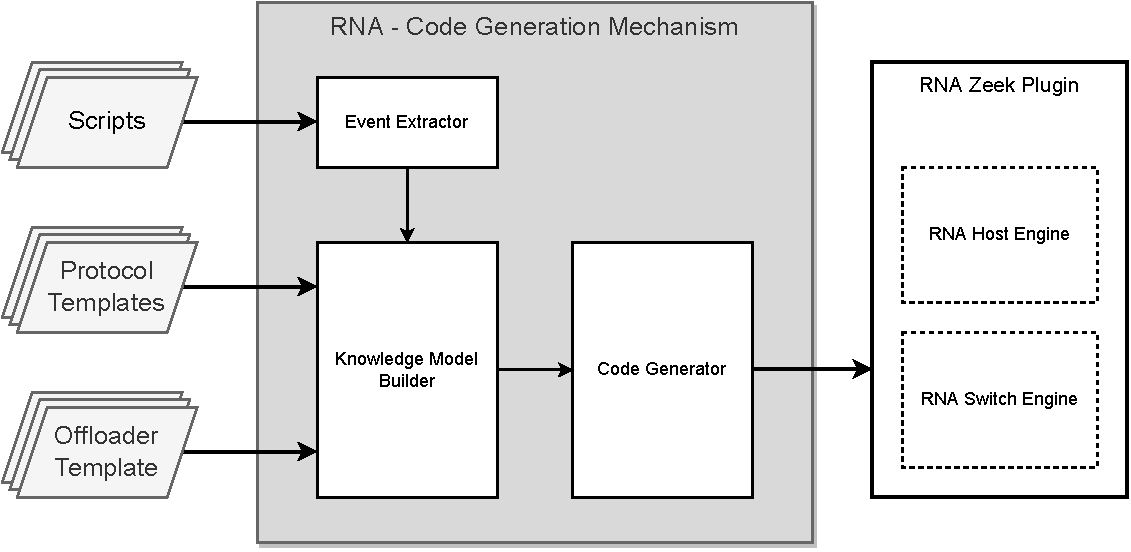
\includegraphics[width=0.98\textwidth]{images/code_gen_mechanism.pdf}
    \end{center}
    \label{fig:code_gen_black_box}
    \legend{Source: the author (2022).}
\end{figure}

The second set of inputs is what we call \textit{templates}, which can be either  Protocol Templates or Offloader Templates. They are a pool of known implementations of protocols and events that can be used to offload scripts. A template being present in this pool does not mean it will be included in the final output, but it means it is available in case its implementation is needed by a script.

The desired output of our mechanism is a single Zeek Plugin following the structure previously presented in \autoref{sec:rna:overview} and illustrated in \autoref{fig:arch_low_level}. This Zeek Plugin, when executed, should: configure the switch, by creating a mirroring session for the Zeek monitoring system and deploying the P4 code; and configure Zeek, by registering all Translators in Zeek's Event Engine, and loading the RNA Event Handler. This eliminates the need for the operator to coordinate the deployment of two separate systems, i.e., the RNA Host Engine and the RNA Switch Engine.

To be able to execute this task, the first objective of the code generation process is to analyze all the provided Zeek scripts and identify which are the observed events in every script. Once this pool of events is known, we select Offloaders (from the templates pool) that are capable of offloading those events. This step is finished and succeeds if we find at least one Offloader for every event.

After all events and Offloaders have been selected, the mechanism must ensure all templates for the protocols required by these Offloaders are available. The Protocol Templates are required so the Offloaders can interpret the desired headers. After all this knowledge model is complete, the mechanism generates all required source files.

Some of the resulting code that is present in the final Zeek Plugin is extracted and merged from the templates, and not completely generated by our mechanism. It is not yet possible to fully generate all offloader code, because the process of converting C++ or P4 code from one to another is very complicated and is out of the scope of this project.


% ==============================================================================
%                            Detailed Mechanism Design
% ==============================================================================

\section{Detailed Mechanism Design}
\label{sec:code_gen:detailed}

The operation of our RNA Code Generation Mechanism can be described in three different stages. The first stage identifies the events that our input scripts subscribe to. The second stage is building our knowledge model, which receives as inputs all Protocol Templates, Offloaders, and events of interest, that the network operator requested to be offloaded. We call this knowledge model \textit{ProtocolGraph}. The last stage is the actual code merge and generation process using this structured and validated knowledge model from the previous step. We start explaining the first stage of our mechanism, i.e., extracting the subscribed events from the Zeek Scripts.

\subsection{Event Extraction}

To identify which events a Zeek Script subscribes to, we first need to parse the script as a whole. The mechanism does it using Zeek's provided grammatical definition. After parsing all the scripts, we search the Abstract Syntax Tree for event handlers, returning their event identifiers. \autoref{fig:event_extraction_example} illustrates a fragment of a Zeek Script that detects FTP Bruteforce attacks. For this particular example, the mechanism would identify the event handler declaration on line $20$, which is the \texttt{ftp\_reply} event.

\begin{figure}[htb]
    \caption{Section of a Zeek Script}
    \begin{center}
        \lstinputlisting[style=zeek]{code/example_zeek_script.zeek.txt}
    \end{center}
    \label{fig:event_extraction_example}
    \legend{Source: the author (2022).}
\end{figure}

In this stage, the most important information to be forwarded to the next step is the identifiers of the events we want to offload. Those will indicate the requirements of our deployment. The name of the scripts are also passed to the knowledge model as a logging and debugging asset but are no longer essential for the final functionality.

\subsection{Knowledge Model Builder}

The core logic behind the implementation of our RNA Code Generation Mechanism relies on a structure we call \textit{ProtocolGraph}. This is a graph structure that stores all protocols required for our events of interest. The Offloaders are linked to their final protocol layer in the graph, generating, in the end, a structure as presented in \autoref{fig:protocol_graph}. This structure is a graph, with a node we assign as root, in most cases, the \textsc{Ethernet} protocol. The other protocols are linked to their respective parents. The Offloaders are linked to the protocol they analyze, which does not need to be a leaf protocol.

\begin{figure}[htb]
    \caption{Knowledge Model - Protocol Graph}
    \begin{center}
        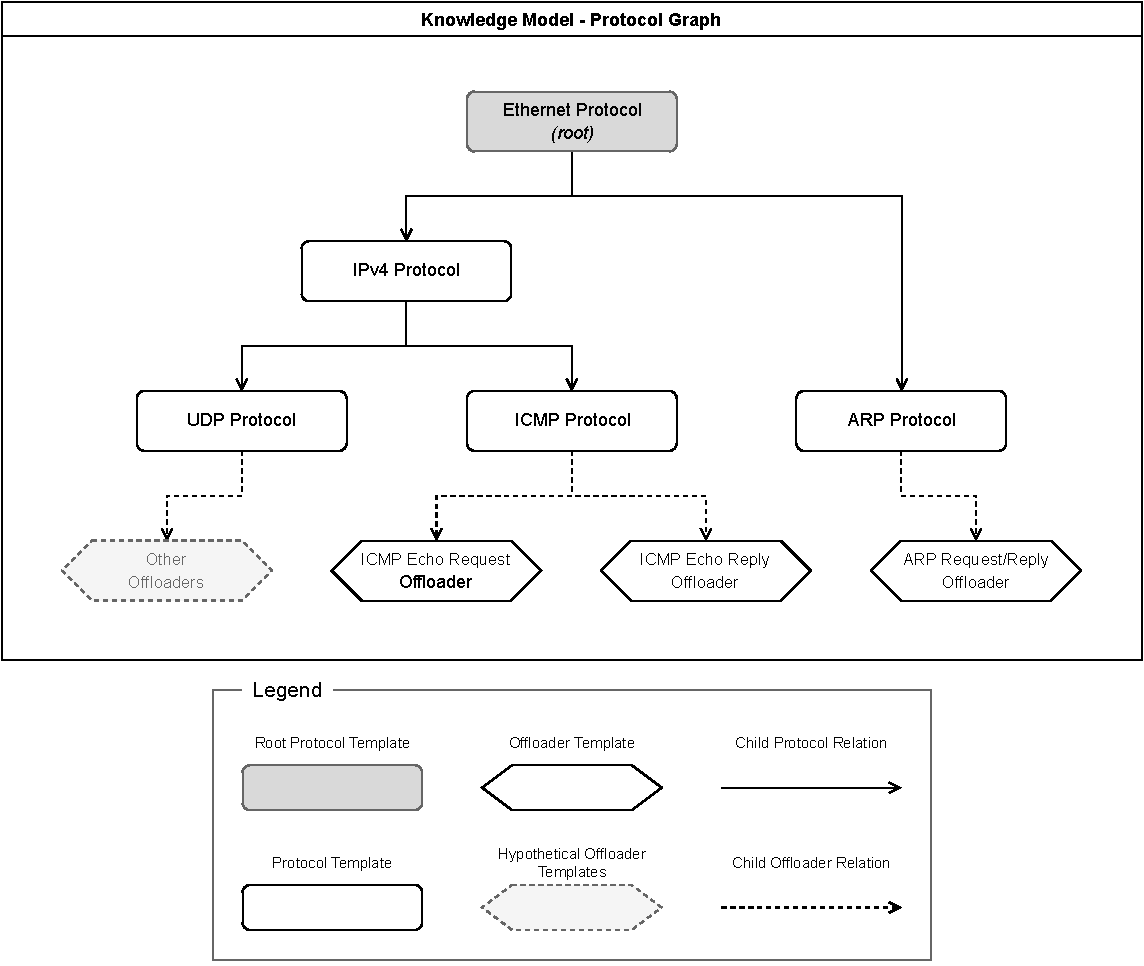
\includegraphics[width=0.98\textwidth]{images/icmp_ex_protocol_graph.pdf}  
    \end{center}
    \label{fig:protocol_graph}
    \legend{Source: the author (2022).}
\end{figure}

The procedure to generate and validate the \textit{ProtocolGraph} is outlined in \autoref{alg:build_graph}. The pseudo-code will be used to describe and guide the explanation of our method and we will refer to the lines according to their respective roles.

\begin{algorithm}[htb]
    \caption{Knowledge Model Build Algorithm}
    \label{alg:build_graph}
    \SetKwInput{Input}{Input}
    \SetKwInput{Output}{Output}
    
    \Input{$templates$, $events$, $forced\_of\!floaders$}
    \Output{$graph$}
    
    \vspace{1em}

    \Call{ValidateComponentList}{$templates$}

    \vspace{1em}

    $protocols \gets$ FilterListByType($templates$, $ProtocolTemplate$) \\
    $of\!floaders \gets$ \Call{FilterListByType}{$templates$, $Of\!floaderTemplate$} \\
    
    \vspace{1em}
    
    $of\!floaders \gets$ \Call{ReqOffloaders}{$of\!floaders$, $events$, $forced\_of\!floaders$} \\

    \vspace{1em}

    \If{$of\!floaders$ is empty} {
        \textbf{raise} \textit{exception} \Comment{nothing to be offloaded}\\
    }

    \vspace{1em}

    $root \gets$ \Call{FindRootProtocol}{$protocols$} \\
    $graph \gets$ \Call{LinkGraph}{$root$, $protocols$} \\

    \vspace{1em}

    \If{\Call{HasCycles}{$graph$}} {
        \textbf{raise} \textit{exception} \Comment{protocol graph has cycles}\\
    }
    
    \vspace{1em}
    
    $protocols \gets$ \Call{RemoveUnreachableProtocols}{$graph$, $protocols$} \\
    \Call{AttachOffloaders}{$graph, of\!floaders$} \\
    
    \vspace{1em}

    \Call{TrimUnusedProtocols}{$graph$} \\
    
    \vspace{1em}
            
    \Call{SetProtocolDepths}{$graph$} \\
    \Call{SortProtocols}{$graph$} \\
    \Call{SortOffloaders}{$graph$} \\
    \Call{SetOffloadersUids}{$graph$} \\
    
    \vspace{1em}
            
    \textbf{return} $graph$ \Comment{successful graph generation} \\
    % \legend{Source: the author (2022).}
\end{algorithm}


\subsubsection*{Template loading and filtering}
% Lines 1 - 6

As the mechanism is executed, the first step is to load all templates and validate their versions, files, and requirements. All the templates are loaded and stored in a list, even if they are not used later in the final model. After they are loaded, we separate them between Protocol Templates and Offloader Templates (\autoref{alg:build_graph}, lines 1-3).

After all offloader templates are validated, we select what offloaders are required (line 4). This selection process is based on two parameters: the event identifiers (provided by the Event Extraction stage), and a list of ``forced'' offloaders (provided by the network operator when invoking the code generator mechanism). The first offloaders to be assigned as required are the ones explicitly requested by the network operator. Next, we select an offloader for each event, making sure all events are covered. If at the end of this process, one or more events do not have offloaders associated with them, the process fails and is aborted. Otherwise, we proceed. We then check if the list of Offloaders is not empty and proceed to the next section (lines 5-6).

\subsubsection*{Graph building}
% Lines 7 - 13

After the templates have been validated and the desired Offloaders have been selected, the mechanism needs to find the root protocol. If none or more than one root Protocol Template is found, an exception is raised and the process is terminated (line 7).

Each Protocol Template has its own identifier, which is a unique string, as well as the identifiers of the parent protocols. Using these identifiers, the Protocol Templates are linked to their parent, making sure the links are all valid (line 8), for example, the ICMP protocol is linked to its parent protocol, the IPv4. After linking, the algorithm validates there are no cycles on the protocol graph (lines 9-10). The reason the protocol graph can not have cycles is due to limitations on the algorithm's P4 implementation, where protocol headers can not be parsed twice for a single packet. By ensuring no cycles are present in the \textit{ProtocolGraph}, we ensure protocol headers can only be used once. After the graph is built, the algorithm removes all unused protocols from the protocol list (line 11).

The algorithm links all the required Offloaders to their respective protocols (line 12). If any Offloader fails to be attached to its protocol, the algorithm aborts the execution. At this point, the \textit{ProtocolGraph} is fully built, but it may have unnecessary protocols still attached to it. These protocols that have no Offloaders attached to them or any Offloaders attached to their child protocols are removed on line 13. It might sound strange that we build the graph, to then trim and optimize it. Since the development of this mechanism was incremental, this is how it was originally developed, but we acknowledge it could be further optimized.

We acknowledge that this implementation is not the optimal implementation and that it could be further optimized.

\subsubsection*{Sorting and Prioritization}
% Lines 14 - 17

After the \textit{ProtocolGraph} is fully built, the mechanism sets the last metadata that will be needed in the code generation stage. The first metadata to be set is the \textit{protocol depth}. For each protocol, the mechanism sets protocol depth as the maximum distance of that protocol to the root protocol (line 14). The depth is used to then sort the protocols and their Offloaders in a list (lines 15 and 16), which will later be consumed by the code generator. A list based on Offloader priority is also created at this time. The last step is to set the unique identifier (UID) for the Offloaders (line 17). This ensures the Switch Engine and the Host Engine have the same identifier referring to the same Offloaders.

\subsection{Code Generation}

The code generation is based on a \textit{master template} with blank slots, which are filled with the generated code. The code that fills the slots of the master template is either fully generated by the mechanism, or is pulled from the protocol and Offloader templates.

Next, we first describe how the code is generated for the P4 switch, then we describe how it is generated for the Zeek Plugin. This code generation process could be in most parts parallelized since it is based on the previously generated \textit{ProtocolGraph}, but we did not see the necessity to implement the parallelism at this time.

\subsubsection*{Code Generation for the Programmable Switch (P4)}

The P4 code is mainly composed of three files, which are \textit{headers.p4}, \textit{parser.p4}, and \textit{main.p4}. We explain this structure in a bottom-up approach, starting with the headers file. The headers file, as the name suggests, contains all the headers and data structures required by the output program. It is generated by merging all headers provided by the templates, which include protocol headers, mRNA headers, and Offloader specific headers\footnotemark{}, and others. In this file, the mechanism also generates \textcolor{blue}{the structure that holds all headers, this is where parsed protocol headers will be saved for each packet}. This structure is generated using the previously-sorted lists of protocols and offloaders because the protocols need to be inserted into the structure according to their layering order. The first header to be included is the root protocol, followed by the rest of the protocols (starting with lower-layer protocols), then the mRNA headers, and finally the Offloader-specific headers, which are the last ones to be added.

\footnotetext{The Offloader specific headers are headers created by the Offloader Splicer, which were explained in \autoref{sec:rna:detailed_design}.}

The \textit{parser.p4} file contains all the information required for parsing and deparsing protocols. The parser, as described previously in \autoref{sec:rna:detailed_design}, is a state machine. The states of the parser are all generated based on the information provided by the protocol templates. It uses the next protocol selector field to select one of the child protocols. Using our example from \autoref{sec:rna:detailed_design}, shown in \autoref{fig:icmp_ex_parser}, the Ethernet parsing state would use the \texttt{ethernet.ethertype} field to select either the \textit{IPv4} or \textit{ARP} protocols. When parsing our example \textsc{ICMP Echo Request} packet, the value of the ethertype field would point to IPv4. Likewise, the value of the \texttt{Protocol} field in the IPv4 datagram would point to ICMP.

To support protocols with variable-size headers, the template has the option to use a custom parsing code, which replaces the default header extractor. Instead of extracting a fixed-size header, based on a (fixed-size) structure, this custom code allows the templates to determine the received header size, and parse the right amount of bits from the packet.

For deparsing and sending an mRNA message, the mechanism does not need to generate any complex code. Since all our headers have already been sorted in our header holding structure (defined in the \textit{headers.p4} file), all the mechanism needs to do is to generate an \textit{emit} command with all headers of a packet. When this code is executed, the P4 switch will check and emit only valid protocols, eliminating the need for us to generate a code section checking the validity of each protocol.

The main P4 file is the entry point for our P4 program. It defines the ingress and egress pipeline control structures, while also loading the headers and the parser files. When generating the ingress pipeline, we split it into two generated sections, the \textit{protocol preprocessors}, and the \textit{Offloader triggers}. The protocol preprocessors section is generated by merging the preprocessors provided by every protocol template, which were explained in \autoref{sec:rna:detailed_design}. The preprocessors are each wrapped with verification to ensure the protocol is valid for that packet, and are generated in bottom-up order. \autoref{fig:ingress_pipeline_ex} shows an example of a section of the ingress pipeline. The generated protocol preprocessors are displayed on lines 3 - 16, where each of the preprocessors is wrapped with an \textit{if statement} to ensure the protocol is valid before executing the preprocessor.

Still in the ingress pipeline, the Offloader triggers are conditions provided with every Offloader template and are also wrapped with a test for protocol validity. They are sorted based on the Offloader's priority, since only one Offloader may be triggered per packet. This is an if statement, which when met, sets the \texttt{metadata.offloader} field to the Offloader's UID, which is defined in the \textit{ProtocolGraph}. Using \autoref{fig:ingress_pipeline_ex} again as an example, on lines 20 - 39 the Offloader triggers are defined. The trigger condition for the \textit{NTP Message Offloader} is seen on line 26. If this condition is true, the P4 switch will set the \texttt{meta.offloader\_type} field to \texttt{RNA\_NTP\_MESSAGE\_UID} (line 27).


\begin{figure}[htb]
    \caption{Section of the P4 Ingress Pipeline}
    \begin{center}
        \lstinputlisting[style=p4]{code/ingress_pipeline.p4.txt}
    \end{center}
    \label{fig:ingress_pipeline_ex}
    \legend{Source: the author (2022).}
\end{figure}

Still in the \textit{main.p4} file, the egress pipeline is composed of one generated section, the \textit{Offloader splicers}. This code section is composed of \textit{if} statements verifying the metadata's Offloader identifier. In the \textit{if} body, the mechanism merges the splicer code, which is provided by every Offloader template and will be executed if the Offloader UID matches the one in the metadata. \autoref{fig:egress_pipeline_ex} shows an example of the splicer section of the egress pipeline. Lines 2 and 6 verify the triggered offloader, and lines 3 - 5, and 7 - 9 are the splicer code for the \textit{FTP Message Offloader} and the \textit{NTP Message Offloader} respectively.

\begin{figure}[htb]
    \caption{Section of the P4 Egress Pipeline}
    \begin{center}
        \lstinputlisting[style=p4]{code/egress_pipeline.p4.txt}
    \end{center}
    \label{fig:egress_pipeline_ex}
    \legend{Source: the author (2022).}
\end{figure}

\subsubsection*{Code Generation for the Zeek Plugin package}

The generation of the Zeek Plugin is much simpler than the P4 code generation. Most of the Zeek Plugin is composed of static files, which are copied from the \textit{master template} and from the templates. The rest of the generation consists of registering the template's Analyzers, defining constants, and creating \textit{read me} and \textit{version} files.

The most important files to be generated are the main plugin file (\texttt{Plugin.cc}), the main Zeek Script file (\texttt{main.zeek}), and the building rules (\texttt{CMakeLists.txt}). The main plugin file needs to include the C++ header files and register the Analyzers. The main Zeek Script file needs to contain instructions to load the Analyzers and bind them to the specific Offloader UIDs, which were defined by the \textit{ProtocolGraph}. To ensure all the template's code files are properly compiled, the mechanism needs to add all their file paths to the \textit{CmakeLists} recipe. The last step in the composition of the Zeek Plugin package is to generate the \texttt{README} file, which describes what the plugin does, and the \texttt{VERSION} file, which contains the version of the generated plugin.

The proposed mechanism was conceived to embed the P4 code in the Zeek Plugin package so that when the RNA Manager is initiated, the P4 code can be deployed to the programmable forwarding device. This was not implemented in the prototype, but we briefly describe how it could be implemented. This could be implemented by first generating the P4 code, then compiling it, either with a P4 command or even in a Docker container to ensure all dependencies are met. After that, when generating the Zeek Plugin package, the mechanism would embed the output of the P4 code compilation (a \textit{JSON} file), and generate a function to load it to the switch when the RNA Manager were initialized.

